\documentclass{beamer}

\usepackage[utf8]{inputenc}
\usepackage{graphicx}
\usepackage{xcolor,colortbl}
\usepackage{subfigure}
\usepackage{hyperref}
%\usepackage{columns}
\usepackage{default}
\usetheme{Frankfurt}
\usecolortheme{seahorse}

\setbeamertemplate{footline}[page number]


%\usecolortheme{whale}
\centerline{
\includegraphics[scale=0.4]{../images/easy_elua_logo}}

\title{Projet innovant RICM4: Easy-eLua}
\author{Elizabeth \textsc{Paz} \\ Salem \textsc{Harrache}}
\institute{Polytech'Grenoble \\
Olivier \textsc{Richard} \\
Didier \textsc{Donsez} \\
}

\author[Elizabeth Paz, Salem Harrache]
{Elizabeth Paz \and Salem Harrache}

\pgfdeclareimage[height=1cm]{university-logo}{../images/polytech.png}
\logo{\pgfuseimage{university-logo}}
\date{27 Avril 2012}

\begin{document}


\begin{frame}
 \maketitle
\end{frame}

\begin{frame}
\frametitle{Sommaire}
\tableofcontents
\end{frame}

\section{Introduction}
\subsection{Présentation carte STM32F4-DISCOVERY}
\begin{frame}
\frametitle{Introduction : Présentation carte STM32F4-DISCOVERY}
Partie Elizabeth 

Note salem : présenter brivement les caracteristiques et puis finir sur le fait que 
c'est compliqué de programmer dessus pour un novice
\begin{center}
 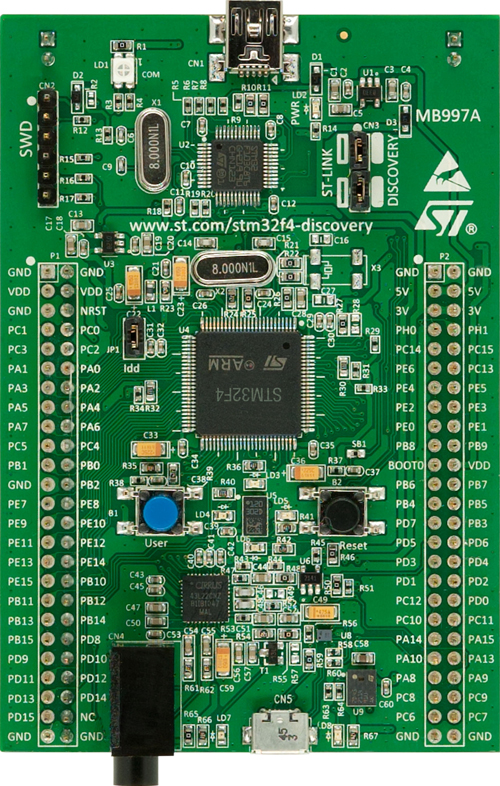
\includegraphics[scale=0.1]{../images/stm32f4_discovery.jpg}
\end{center}
\end{frame}

\subsection{Présentation Arduino}
\begin{frame}
\frametitle{Introduction : Présentation Arduino}
Partie Elizabeth 
Note salem : Le site est bien fait, puis y a des presentation sur internet de la carte 
donc easy. Dire qu'il y a deux methode a implementer (loop et setup) et puis un point sur
l'open source. Meme les carte en elle meme sont open source, ce qui est vraiment appreciable
pour tout ingenieurs qui veut se lancer dans un nouveau projet etc...
\begin{center}
 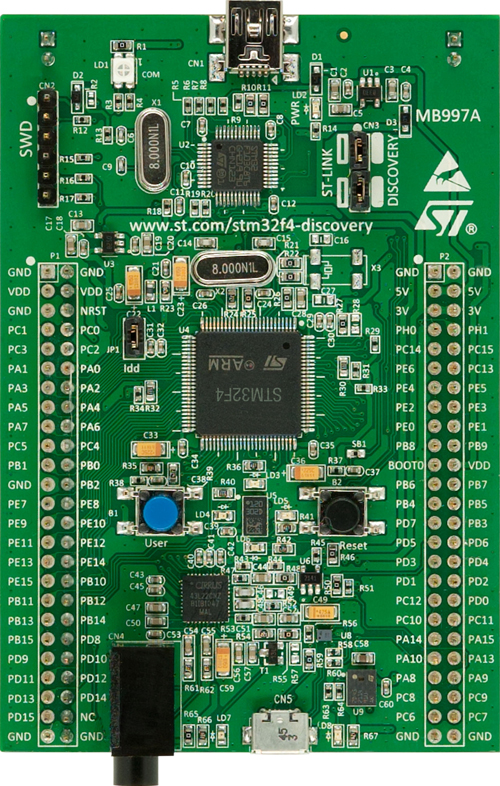
\includegraphics[scale=0.1]{../images/stm32f4_discovery.jpg}
\end{center}
\end{frame}

\subsection{Présentation eLua}
\begin{frame}
\frametitle{Introduction : Présentation eLua}
partie Elizabeth

\url{http://www.eluaproject.net/overview} + 
architecture : \url{http://www.eluaproject.net/doc/v0.8/en_arch_overview.html}


la utilise le schéma et dis que notre mission c'etait d'evaluer le portage, et dire 
qu'on a contacté ton James (xD) et qu'on a reussis a le faire travailler pour nous xD

C'est important je pense de le mentionner :)
\begin{center}
 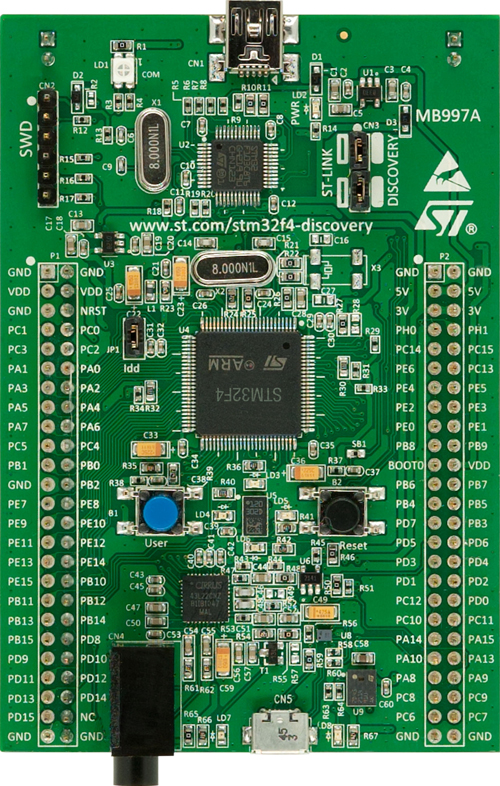
\includegraphics[scale=0.1]{../images/stm32f4_discovery.jpg}
\end{center}
\end{frame}

\section{Travail réalisé}
\subsection{Organisation du travail}
\begin{frame}
\frametitle{Introduction : Organisation du travail}
à faire par Salem
\begin{center}
 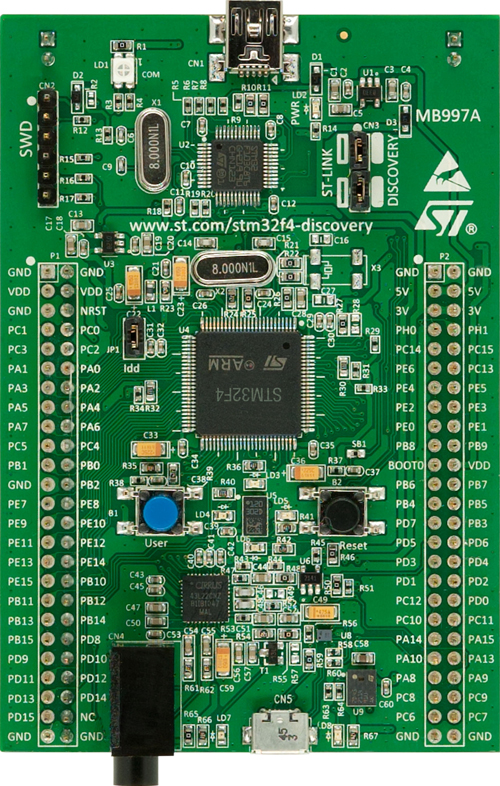
\includegraphics[scale=0.1]{../images/stm32f4_discovery.jpg}
\end{center}
\end{frame}

\subsection{Arboresence du projet}
\begin{frame}
\frametitle{Arboresence du projet}
à faire par Salem
\begin{center}
 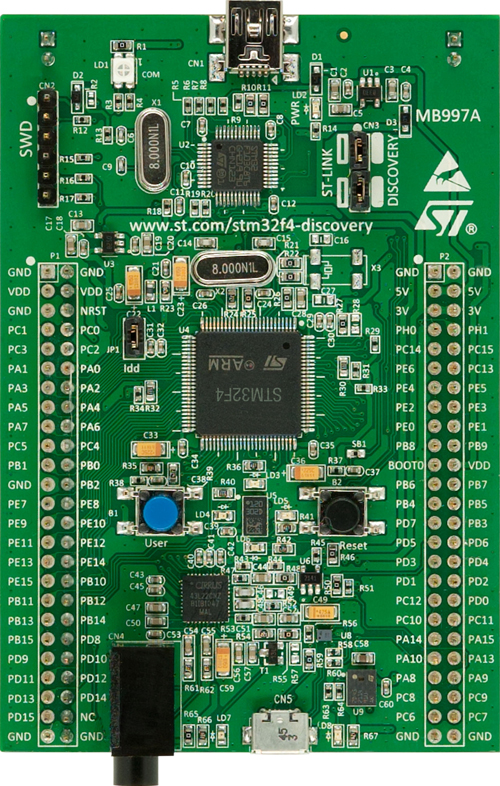
\includegraphics[scale=0.1]{../images/stm32f4_discovery.jpg}
\end{center}
\end{frame}

\subsection{Fonctions portées}
\begin{frame}
\frametitle{Fonctions portées}
à faire par Salem
\begin{center}
 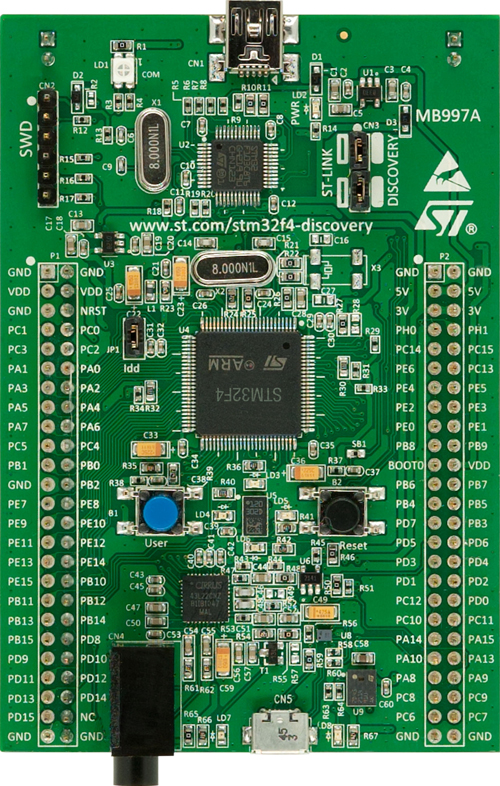
\includegraphics[scale=0.1]{../images/stm32f4_discovery.jpg}
\end{center}
\end{frame}

\subsection{Nouveaux concepts}
\begin{frame}
\frametitle{Nouveaux concepts}
à faire par Salem
\begin{center}
 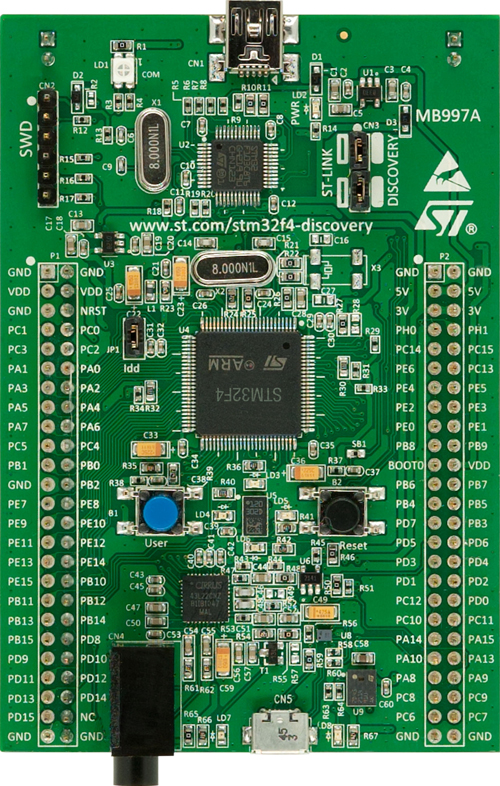
\includegraphics[scale=0.1]{../images/stm32f4_discovery.jpg}
\end{center}
\end{frame}

\section{Demonstration}
\subsection{``Hello Word!''}
\begin{frame}
\frametitle{Demonstration : ``Hello Word!'' avec flash}
à faire par Salem et expliquer à Elizabeth
\begin{center}
 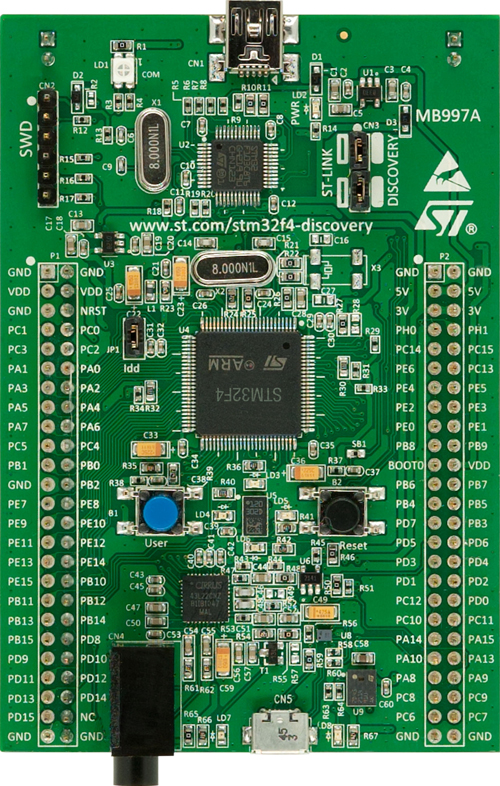
\includegraphics[scale=0.1]{../images/stm32f4_discovery.jpg}
\end{center}
\end{frame}

\subsection{``Blink with button''}
\begin{frame}
\frametitle{Demonstration : ``Blink with button'' avec le shell}
à faire par Salem
\begin{center}
 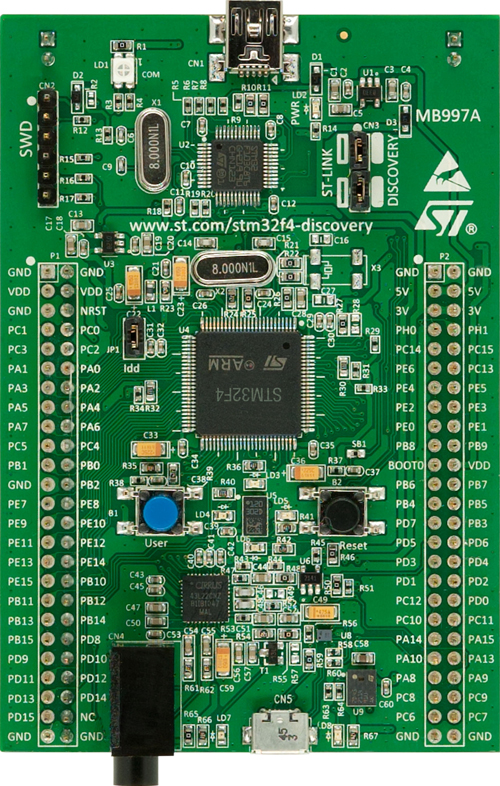
\includegraphics[scale=0.1]{../images/stm32f4_discovery.jpg}
\end{center}
\end{frame}

\subsection{``Ascii table''}
\begin{frame}
\frametitle{Demonstration : Lancement de script sans flash}
à faire par Salem
\begin{center}
 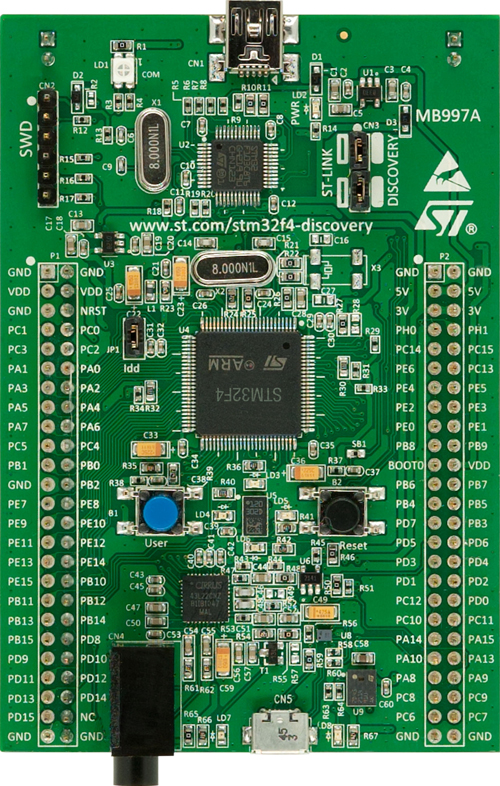
\includegraphics[scale=0.1]{../images/stm32f4_discovery.jpg}
\end{center}
\end{frame}

\section{Conclusion}
\subsection{Difficulté}
\begin{frame}
\frametitle{Conclusion : Difficulté}
à faire par Salem ou Elizabeth
\begin{center}
 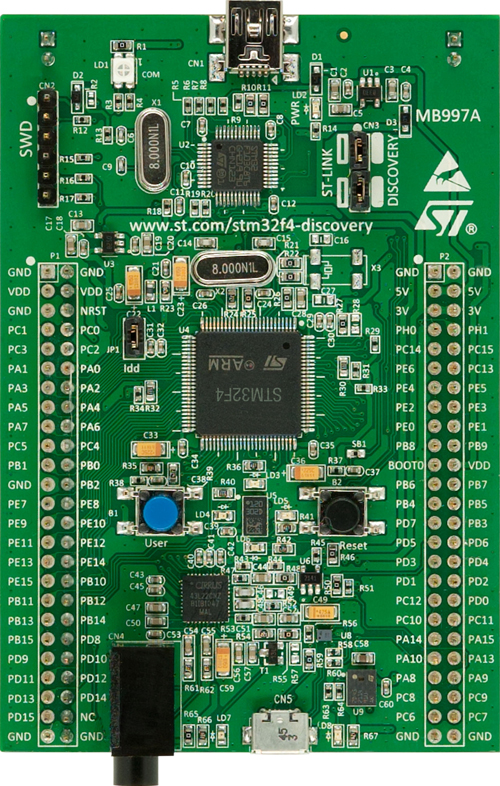
\includegraphics[scale=0.1]{../images/stm32f4_discovery.jpg}
\end{center}
\end{frame}

\subsection{Bilan}
\subsection{Difficulté}
\begin{frame}
\frametitle{Difficulté du projet}
à faire par Salem ou Elizabeth
\begin{center}
 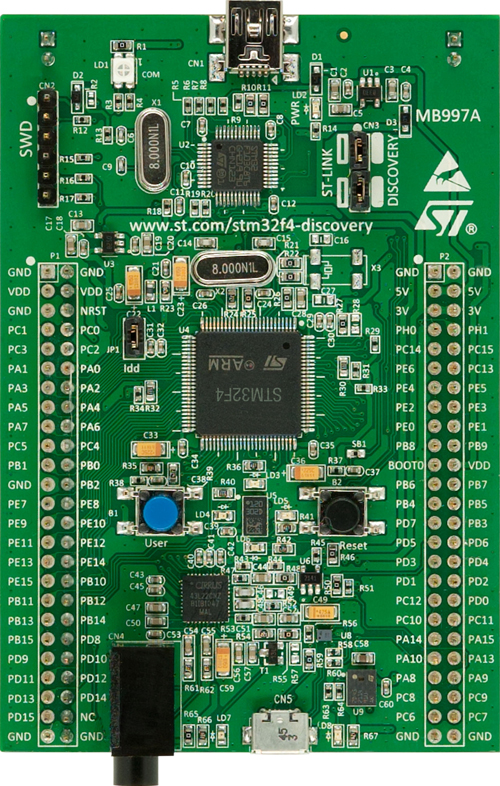
\includegraphics[scale=0.1]{../images/stm32f4_discovery.jpg}
\end{center}
\end{frame}

\subsection{Bilan}
\begin{frame}
\frametitle{Bilan}
à faire par Elizabeth ou Salem
\begin{center}
 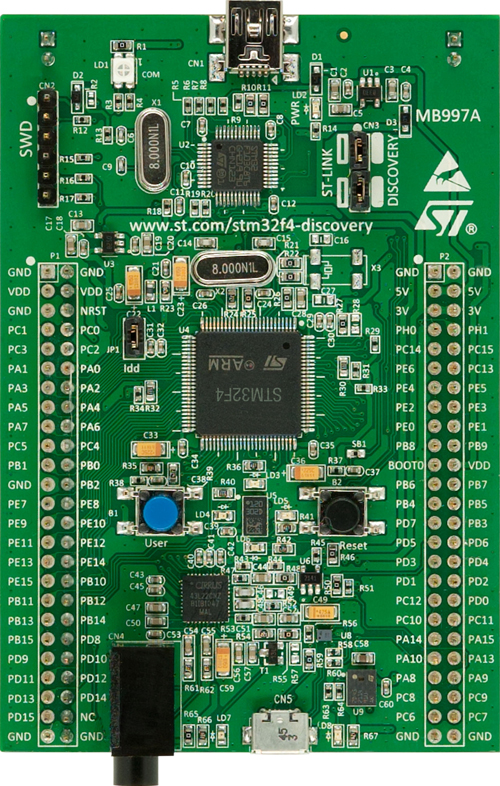
\includegraphics[scale=0.1]{../images/stm32f4_discovery.jpg}
\end{center}
\end{frame}

\begin{frame}
\frametitle{Conclusion}
\begin{center}
\huge{Des questions ?}
\end{center}
\end{frame}

\end{document}